\section{Drei-Ebenen-Model des kooperativen und autonomen Fahrens}
\label{ch_3EM}
In Anlehnung an~\cite{Rasmussen1983} und~\cite{Donges1982} unterteilen wir die Fahraufgabe in die  \textit{Navigationsebene},  \textit{Bahnführungsebene} und  \textit{Fahrzeugführungsebene}.

In der \textit{Navigationsebene} werden neben der klassischen Aufgabe der Vorausplanung einer Fahrstrecke auch diskrete Entscheidungen innerhalb von Einzelfunktionen durchgeführt wie z.B. Parklücke links oder rechts wählen, Spur wechseln oder in der Spur verzögern, links oder rechts abbiegen, usw..

In der \textit{Bahnführungsebene} wird die durch die Navigationsebene vorgegeben Fahraufgabe umgesetzt.  Dabei muss das Fahrzeugumfeld berücksichtigt werden (prädizierte Objektbewegungen, Randbebauungen, etc.) und sichergestellt werden, dass die Fahrbarkeit anhand des Potenzials des Fahrzeugs gewährleistet ist. Die Bahnführungsebene ist fahrzeugparameterfrei und kennt nur die geometrischen Ausmaße der Fahrzeugkarosserie, um Kollisionsfreiheit prüfen zu können. Eine Trajektoriefolgeregelung längs und quer regelt geometrische Abweichungen von der Solltrajektorie bspw. aufgrund von Störungen aus und generiert als fahrzeugparameter- und geschwindigkeitsunabhängige Vorgaben der Quer- und Längsführung eine Sollkrümmung und eine Solllängsbeschleunigung für die unterlagerte \textit{Fahrzeugführungsebene}. Die Trajektoriefolgeregelung längs und quer erfolgt hierbei getrennt, +schlauer Halbsatz.

Das Potenzial, welche Trajektorien fahrbar sind, wird durch die unterlagerte \textit{Fahrzeugführungsebene} die die vollständige Information über die verbauten Sonderausstattungen, das Potenzial der Aktuatoren, der Fahrdynamik, Fahrzustandsbeobachter, Fahrzeugparameterschätzer, usw. besitzt und als abstrahierte Potenzialbeschreibung für eine mögliche Fahrzeugbewegung bereitstellt. In der \textit{Fahrzeugührungsebene} werden die fahrzeugparameterfreien Sollvorgaben Sollkrümmung und Längsbeschleunigung eingeregelt und die Aktuatoren angesteuert.
Hierbei ist es Aufgabe der kooperativen Fahrzeugführungsregelung quer und längs zum einen, ein möglichst gutes Führungsübertragungs- und Störübertragungsverhalten darzustellen,
und zum anderen die Fahrereingaben, im Sinne der beispielhaft für die Querführung in Abb.~\ref{fig:koopgrad} beschriebenen Kooperationsgrade, mit zu berücksichtigen. 

Abb.~\ref{fig:3EM} zeigt hierzu stark vereinfacht und schematisiert die angenommene Struktur eines Drei-Ebenen-Modells für manuelles, kooperatives und autonomes Fahren.
\begin{figure}[htp!]
  \centering
    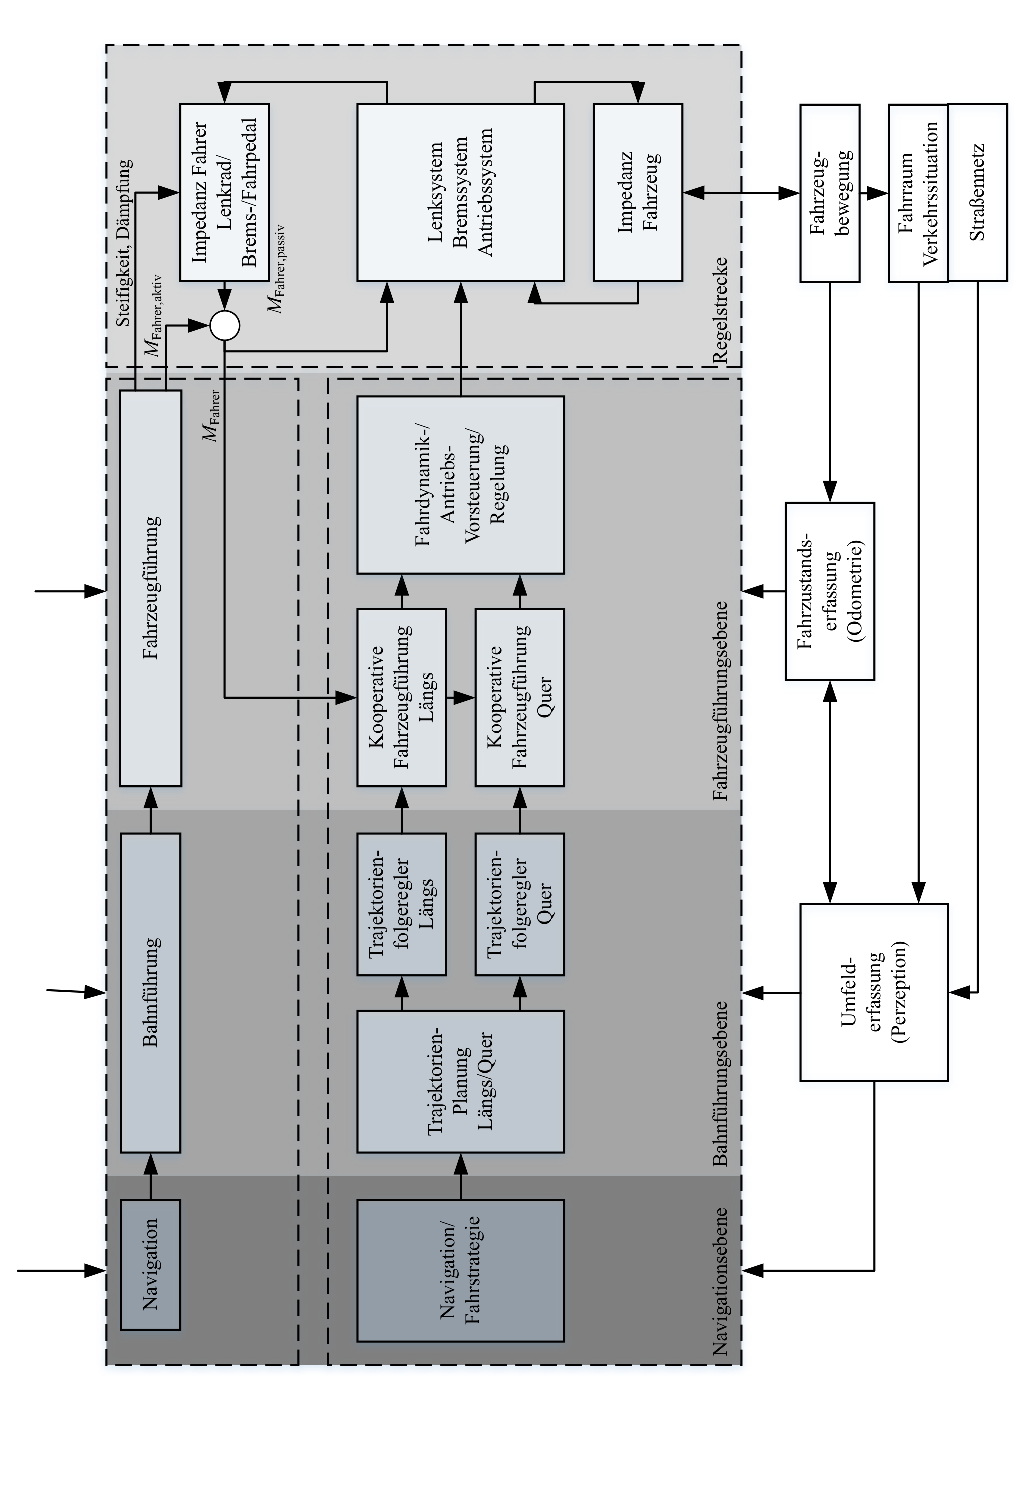
\includegraphics[scale=0.7]
    {Bilder/01/3EM.eps}
    \caption{Adaptiertes Drei-Ebenen-Modell für integrierte Quer- und Längsführung}
    \label{fig:3EM}
\end{figure}
Ausgangsseitig ist die Bahnführungsebene direkt an die Aktuatorregelungen der Fahrzeugführung angegliedert. Für die Querführung wird dabei als Schnittstelle eine umzusetzende Sollkrümmung $\kappa_\mathrm{d}$ übergeben.  Diese bietet den Vorteil der Unabhängigkeit von der Fahrzeuggeschwindigkeit. Damit sind Parkier- und Fahrfunktionen mit der gleichen Schnittstelle bedienbar. Des Weiteren ergibt sich eine Unabhängigkeit von verwendeten Aktuatorik auf der Bahnführungsebene: Innerhalb der Fahrzeugführungsebene können Vorderachs- und Hinterachslenkungen verwendet werden oder gegebenenfalls einseitige Bremseingriffe zur Erzeugung eines Giermoments, um die geforderte Sollkrümmung umzusetzen.\\ 
Bei der Längsführung wird eine Sollbeschleunigung $a_\mathrm{d}$ übergeben. Diese wird in ein Sollradmoment umgerechnet und je nach Betriebsbereich auf die beiden Aktuatoren Antrieb und Bremse verteilt. 

Im Rückkanal liefert die Fahrzeugführungsebene der Bahnführungsebene das ermittelte zur Verfügung stehende fahrdynamische Potenzial.  Dieses wird in abstrahierter Form bereitgestellt. Dazu werden geometrische Grenzen, Aktuatorgrenzen, physikalische Grenzen und Grenzen die aus der Funktionalen Sicherheit resultieren berücksichtigt.\\
Den Reifen eines Fahrzeugs kommt bei der Kraftübertragung eine entscheidende Rolle zu. Je nach Reibwert können diese nur eine bestimmte Kraft übertragen. In dynamisch unkritischen Situationen stellt sich der Kraftaufbau dabei linear zum anliegenden Schlupf ein. In hochdynamischen Situationen oder bei niedrigem Reibwert ist das Übertragungsverhalten allerdings gesättigt. Eine genaue Identifikation des Übertragungsverhaltens ist schwierig und immer noch Gegenstand der Forschung. Um nicht für jeden Reifen die Kennlinie einzeln identifizieren zu müssen, werden deshalb die idealisierten Zusammenhänge nach dem Kamm'schen Kreis verwendet. Dieser erlaubt eine Abschätzung der umsetzbaren Längs- und Querkräfte am Rad eines Fahrzeugs \cite{Risch2002}. Demnach kann die resultierende Kraft $\mathbf{F}_i$ eines Reifens nicht das Produkt aus dem Reibwert $\mu$
und der Normalkraft $F_{n,i}$ überschreiten:
\begin{equation}
|\mathbf{F}_i|= \sqrt{F_{q,i}^2 + F_{l,i} ^2} \leq \mu \, F_{n,i} \text{ mit } i \in [\text{vorne links}, \text{vorne rechts}, \text{hinten links}, \text{hinten rechts}]
\label{eq_kammscher_kreis}
\end{equation}
$F_{q,i}$ und $F_{l,i}$ stellen dabei am jeweiligen Rad die Quer- und Längskomponente der Kraft dar. Wird Bedingung (\ref{eq_kammscher_kreis}) eingehalten, so wird das Rad stets rollen und nicht in den Gleitzustand gelangen \cite{Mitschke2004}.
Da der Reibwert nicht direkt gemessen werden kann, müssen Schätzverfahren zur Ermittlung eingesetzt werden. Zur Reibwertschätzung stehen mittlerweile verschiedene Verfahren bereit, die auch bereits industrialisiert worden sind.\\
Da bei der Planung der zu fahrenden Trajektorien meist das Fahrzeug als Massenpunkt betrachtet wird, das heißt die einzelnen Räder nicht betrachtet werden, kann der Zusammenhang (\ref{eq_kammscher_kreis}) für das gesamte Fahrzeug auf Beschleunigungsebene betrachtet werden:
\begin{equation}
 \sqrt{a_x^2+a_y^2} \leq \mu \, g = a_{pot}
\end{equation}
Demnach ergibt sich die resultierende maximal fahrbare Beschleunigung $a_{pot}$ aus dem Reibwert und der Erdbeschleunigung $g$. $a_x$ beschreibt die Fahrzeuglängs- und $a_y$ die Fahrzeugquerbeschleunigung.
Für die Planung einer fahrbaren Trajektorie ist allerdings nicht der aktuelle Reibwert, sondern der zukünftige Reibwert relevant. Dies macht eine prädiktive Schätzung auf Basis von Umfeldsensorik nötig (siehe z.B. \cite{daniel2014reibwertschaetzung}).\\
Oft beschränkt nicht der Reibwert die fahrbare Trajektorie, sondern die unterlagerten Aktuatoren (gewöhnlich Antrieb, Bremse und Lenkung). Diese weisen konstruktionsbedingte Stellgrößenbegrenzungen auf oder aus Sicherheitsgründen werden ihre Stellraten- und/oder Stellgrößen auf für den Fahrer beherrschbare Werte begrenzt.\\
Bei der Querführung sind hierbei die Endanschläge der Lenkung zu berücksichtigen. Diese führen dazu, dass das Fahrzeug nicht beliebig kleine Radien fahren kann und stellen somit eine Sättigung der umsetzbaren Krümmung dar. Diese lässt sich durch die stationäre Verstärkung des Einspurmodells, das in Kapitel~\ref{ch_Modellierung} beschrieben wird, aus dem maximal möglichen Lenkwinkel $\delta_{max}$ berechnen:
\begin{equation}
\kappa_{max}=k_\kappa \, \tan \left(\delta_{max}\right) 
\end{equation}
Die maximal mögliche Krümmung kann mit 
\begin{equation}
a_{y,max} = \kappa_{max} v_x^2 
\end{equation}
und der aktuellen Fahrzeuggeschwindigkeit $v_x$ in eine maximal mögliche Querbeschleunigung $a_{y,max}$ umgerechnet werden.
\\ 
Auch der Antrieb kann nicht jedes beliebige Moment umsetzen. Über Schnittstellen zur Antriebsaktuatorik steht in modernen Fahrzeugarchitekturen allerdings serienmäßig das im aktuellen Gang maximal umsetzbare Radmoment $\tau_{mot,max}$ als Signal zur Verfügung. Dieses kann mittels der geschätzten Fahrzeugmasse $\tilde m$ und dem angenommenen dynamischen Rollradius $\tilde r$ in eine maximal mögliche Längsbeschleunigung $a_{x,mot,max}$ umgerechnet werden:
\begin{equation}
a_{x,ant,max} = \frac{1}{\tilde m \, \tilde r} \tau_{mot,max} 
\end{equation}
Des Weiteren muss bei niedrigem Reibwert die Antriebsart berücksichtigt werden, sodass das Beschleunigungspotenzial in Längsrichtung  bei einem rein front- oder heckgetriebenen Fahrzeug im Vergleich zu einem allradgetriebenen Fahrzeug bei ausreichendem Motormoment weiter beschränkt ist. Darüber hinaus können Fahrwiderstände, die die Fahrzeuglängsdynamik beeinflussen, berücksichtigt werden. So kann beispielsweise, wie in Kapitel~\ref{ch_Fahrzeugführungsebene} beschrieben wird, die aus den Fahrwiderständen resultierende Störbeschleunigung in Längsrichtung $\tilde z_{a_x}$ beobachtet werden und es ergibt sich als Potenzialgrenze in Längsrichtung
\begin{equation}
a_{x,pot} = a_{x,max} + \tilde z_{a_x}.
\end{equation}
Die maximale Verzögerung wird nicht begrenzt, da üblicherweise davon ausgegangen werden kann, dass die Bremsanlage die maximale Verzögerung erreichen kann.
	   \begin{figure}[thpb]
	      \centering
	  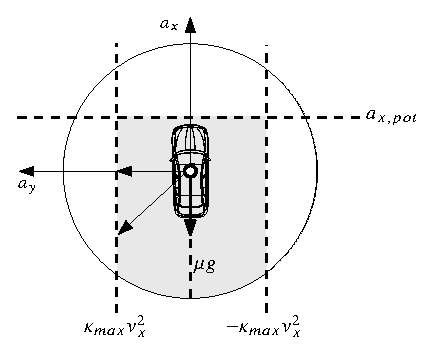
\includegraphics{Bilder/02/pot_vec.eps}
	 \begin{center}
	       \caption{Kamm'scher Kreis mit Begrenzungen.}
	      \label{abb_pot_vec}
	       \end{center}
	   \end{figure} 
%Auf die gleiche Weise wie bei $\kappa_{max}$ und $a_{x,max}$ 
Weiterhin können etwaige Stellratenbegrenzungen $\dot \kappa_{max}$ und $\dot a_{x,max}$ berücksichtigt werden.\\
Abb.~\ref{abb_pot_vec} veranschaulicht die Potenzialgrenzen, die sich aus den Aktuatorbegrenzungen und dem Kamm'schen Kreis ergeben. Die resultierende Beschleunigung der zu planenden Trajektorie darf folglich nur im grau markierten Bereich der Abbildung liegen. Dabei stellen die Grenzen Maximalwerte dar, die auf keinen Fall überschritten werden sollten. Gerade die Schätzung des Reibwerts ist meist nur möglich, wenn bereits großer Schlupf vorliegt. Von daher ist es sinnvoll, die Grenzen als absolutes Maximum zu betrachten und sich ihnen, falls möglich, konservativ zu nähern.\\
Die beschriebenen Größen werden im fahrdynamischen Potenzial zusammengefasst und der Bahnführungsebene zur Verfügung gestellt.\\
 NoNi: zwei geregelte Ebenen, eine gesteuerte! Wichtig Unterscheidung, auf deren Grundlage plausibel wird, dass wir im folgenden nur noch zwei Ebenen betrachten.
\FloatBarrier


\refFig{LongLatOverview} zeigt das Zusammenspiel aller an der integrierten Quer- und Längsregelung beteiligten Softwarekomponenten und Systeme.

%%%%%%%%%%%%%%%%%%%%%%%%%%%%%%%%%%%%%%%%%%%%%%%%%%%%%%%%%%%%%%%%%%
\begin{figure}[htp!]
\centering

\begingroup
\renewcommand*{\arraystretch}{0.75}
\import{Bilder/LongLatOverview/}{LongLat_Overview.pdf_tex}
\endgroup

\caption{Gesamtschau der kooperativen integrierten Längs-Quer-Regelung}
\label{fig:LongLatOverview}
\end{figure}
%%%%%%%%%%%%%%%%%%%%%%%%%%%%%%%%%%%%%%%%%%%%%%%%%%%%%%%%%%%%%%%%%%%


Die Trajektorienplanung (TP) erzeugt auf Grundlage der nicht dargestellten übergeordneten Navigations-/Fahrstrategieebene die Solltrajektorie 
$\begin{bmatrix}x & y & \theta & \kappa & v_x & a_x\end{bmatrix}^T_\mathrm{traj}$. Die nachgelagerten Trajektorienfolgeregler, TC\sus{lat} für die Querbewegung und TC\sus{long} für die Längsbewegung, errechnen aus der Solltrajektorie und der tatsächlichen Lage/Geschwindigkeit
$\begin{bmatrix}x & y & \theta & v_x\end{bmatrix}$ des Fahrzeugs die korrigierenden Stelleingriffe Sollkrümmung $\kappa_\mathrm{d}$ und Solllängsbeschleunigung $a_{x\mathrm{d}}$.

Diese werden durch die beiden Störgrößenbeobachter, DO\sus{$\kappa$} und DO\sus{$a_x$}, so ergänzt, dass beobachtete Störungen stationär kompensiert werden. Die adaptierte Sollkrümmung
$\kappaDPrime$ kann nun durch eine Stellgrößenverteilung (Control Allocation CA\sus{$\kappa$}) auf querdynamisch wirksame Aktuatoren verteilt werden. In den meisten Fällen wird das die Vorderachslenkung oder ein Lenksystem mit aufeinander abgestimmten Vorder- und Hinterachslenkwinkeln sein. Einseitige Bremseingriffe und eine direkte Ansteuerung der Hinterachslenkung sind hier auch denkbar. Der Anteil $\kappa_\delta$ der Sollkrümmung, welcher der Lenkung zugeordnete wurde, wird anschließend in einen Solllenkwinkel $\delta_\mathrm{d}$ umgerechnet. Die adaptierte Solllängsbeschleunigung $\aXDPrime$ wird vor der Verteilung auf Antrieb und Bremse (CA\sus{x}) in ein Sollmoment $\tau_{x\mathrm d}$ umgerechnet. Bei dieser Stellgrößenverteilung werden auch die vom Fahrer (Drv) über Bremspedal (BrkP) und Gaspedal (AccP) kommunizierten Wunschmomente berücksichtigt.

Die so berechneten Brems- und Antriebssollmomente $\tau_\mathrm{brk}$ und $\tau_\mathrm{mot}$ werden an die entsprechenden Aktuatorsteuergeräte übergeben und dort im Wesentlichen ohne Unterscheidung zwischen manuellem oder autonomen Fahren eingeregelt (Brk und Mot; die Blöcke repräsentieren jeweils Steuergerät und Aktuator). Für das Einstellen des Solllenkwinkels $\delta_\mathrm d$ wird im Gegensatz dazu ein zusätzlicher Regler, C\sus{$\delta$}, benötigt, der über die Anforderungen beim manuellen Fahren hinausgeht. 

Antrieb, Bremse und Lenkung (EPS) erzeugen über die Längs- und Querdynamik des Fahrzeugs (Vh\sus{lat} und Vh\sus{long}) die Fahrzeugbewegung, welche durch die tatsächliche Krümmung 
$\kappa$ und die tatsächliche Längsbeschleunigung $a_x$ beschrieben ist. Die dabei physikalisch auftretenden Rückwirkungen auf die Aktuatoren sind in Grau angedeutet.

Der äußere Regelkreis der Trajektorienfolgeregelung schließt sich über die Fahrzeugkinematik (Vh\sus{kin}), die $\kappa$ und $a_x$ zu $\begin{bmatrix}x & y & \theta & v_x\end{bmatrix}$ integriert.

\FloatBarrier

